\documentclass{article}
\usepackage[utf8]{inputenc}
\usepackage{setspace}
\usepackage{hyperref}
\usepackage{url}
\usepackage[T2A]{fontenc}	
\usepackage{ dsfont }
\usepackage{amssymb}
\usepackage[english, russian]{babel}
\usepackage{graphicx}
\usepackage{amsmath}
%\DeclareGraphicsExtensions{.pdf,.png,.jpg}
\usepackage{float}
\usepackage{natbib}
\usepackage{algorithmic}
\usepackage[ruled,vlined]{algorithm2e}
\title{Выбор согласованных моделей для построения нейроинтерфейса}
\author{Кулаков Ярослав}
\date{February 2021}
\doublespacing

\begin{document}

\maketitle




\section{Аннотация}
В работе решается задача построения нейро-компьютерного интерфейса. Требуется предсказать трехмерную траекторию движения кисти по сигналам с коры головного мозга. Сложность задачи состоит в том, что сигнал высокоразмерный и сильно скоррелированный. Предлагается применить методы снижения размерности исходного пространства с согласованием моделей. Для решения задачи используются линейные и нелинейные модели. Анализируются целевое и латентное пространства, получаемые парой моделей. Эксперементальные результаты подтверждают, что предлагаемый метод повышает качество предсказаний модели.

\section{Введение}
Нейрокомпьютерные интерфейсы (BCI) предоставляют возможность интерпретации активности мозга, использовать и обрабатывать ее моделями машинного обучения с целью предсказания действий или декодирования мыслей человека \cite{general_purpose_1300799} \cite{BLANKERTZ20101303}. Из-за высокой сложности мозга и большого количества информации, содержащейся в нем в каждый момент времени, высокой размерности описания данных электроэнцефалограммы и электрокортикограммы. Сигналы представляют собой скоррелированные их временные ряды. Для получения нескоррелированных, но информативных признаков, решается задача снижения размерности исходного пространства.\cite{feature_selection_ecog} \cite{ATYABI2013319} \cite{7330455}
В работе исследуются линейные и нелинейные модели декодирования сигналов. Оценивается качество, устойчивость и сложность рассматриваемых моделей.  \par

В статье \cite{qpfs} проведены сравнения алгоритмов выбора признаков: QPFS \cite{qpfs} с LARS \cite{MICHE20112413}, Lasso \cite{zhao2007stagewise}, Ridge \cite{ridge} и отбор признаков с генетическим алгоритмом \cite{tan2008genetic}. Quadratic Programming Feature Selection \cite{qpfs} показывает наилучшие результаты и этот метод можно адаптировать для нашей задачи. \par
Так же проводится сравнение с методами PLS, PCA, других нелинйных моделей.  При решении задачи выбора признаков, одновременно оптимизируются две задачи: минимизируется корреляция между признаками и максимизируется информативность признаков по отношению к таргету. Задача осложняется тем, что признаки и таргеты имеют разную природу. \par
В данной работе предложен устойчивый алгоритм модулирования сигнала в конечности от состояния активности мозга, состоящий из этапов:
\begin{itemize}
    \item Построение латентного пространства меньшей размерности, с минимальной корреляцией признаков между собой и максимальной корреляцией признаков с предсказываемым сигналом.
    \item Построение прогностической модели в полученном пространстве.
     \item Восстановление обратной зависимости для предсказания активности мозга.
\end{itemize}

\section{Постановка задачи}
Рассматривается выборка $(X, Y).$ $ X \in \mathds{R}^{T, K}$, где $T$ --- количество временных отметок, а $K$ ---  число электродов, используемых для снятия сигнала. $Y \in \mathds{R}^{C, T}$, где $C$ --- номер координаты в трехмерном пространстве. Данные содержат записи о траектории движения руки в трехмерном пространстве и ECoG сигнала. ECoG сигнал снимался с 64х электродов, частотой 1кГц. Чтобы сформировать тензор признаков, каждая эпоха ECoG была сопоставлена с временно-частотно-пространственным пространством с помощью непрерывного волнового преобразования (CWT). %ссыдка
\par
Снижение размерности. Задача состоит в поиске функций $\phi: X^{n\times m} \rightarrow X^{n\times k}$ для объектов и функции  $\psi: Y^{n\times p} \rightarrow X^{n\times q}$ для кодирования целевых переменных. Причем $k < m, q < p.$ Полученные матрицы являются матрицами представлений в латентном пространстве.
\par
 %PLS
\par
Рассматриваются линейные и нелинейные модели. Линейные модели менее подвержены проклятию размерности и слабее переобучаются, а нелинейные методы способны уловить сложные закономерности. Чтобы объединить преимущества обоих методов рассматриваются generalized linear models, additive models и их комбинация --- GAM. \par
Линейная модель задается в виде $\hat y = X^T\theta + \theta_0,$ где $X$ --- матрица объект-признаков, а $\theta$ --- вектор параметров модели. Предполагается, что истинная зависимость так же является линейной, с шумом, распределенным нормально. \par
GLM --- обобщение линейной регрессии, в котором мы можем применять разные функции к $y$, а так же предполагать разные его распределния. \par
AM --- еще один способ по внедрению нелинейности в модель. $\hat y = \theta_0 + \sum \theta_i f_i(x_i)$. \par
Используемые метрики и критерии качества: $MSE(||y-\hat y||_2^2 ), MAE(||y-\hat y||_1), MAPE(\frac{1}{n}\sum \frac{|Y_i-\hat Y_i|}{Y_i})$.  \par
Соответственно задача ставится как минимизация этих Loss-function: $L(X, Y, \Theta) \rightarrow min.$

\section{Теоритическое обоснование}
Определение. Назовём пространство $\mathbb{T} \subset \mathbb{R}^{l}$ скрытым пространством
для пространства $\mathbb{X} \in \mathbb{R}^{n}(l \leqslant n),$ если существуют функция $\varphi_{e}: \mathbb{X} \rightarrow \mathbb{T}$ и
функция $\varphi_{d}: \mathbb{T} \rightarrow \mathbb{X}$ такие что
$$
\mathbf{x} \in \mathbb{X} \quad \exists \mathbf{t} \in \mathbb{T}: \varphi_{d}\left(\varphi_{e}(\mathbf{x})\right)=\varphi_{d}(\mathbf{t})=\mathbf{x}
$$
Функция $\varphi_{e}(\mathbf{x})$ называется функцией кодирования объекта $\mathbf{x},$ функция $\varphi_{d}(\mathbf{t})$
называется функцией декодирования.

Аналогично введём определение скрытого пространства $\mathbb{U} \subset \mathbb{R}^{s}$ для целевого пространства $\mathbb{Y}$, функции кодирования $\psi_{e}: \mathbb{Y} \rightarrow \mathbb{U}$ и декодирования
$\psi_{d}: \mathbb{U} \rightarrow \mathbb{Y}$
$$
\mathbf{y} \in \mathbb{Y} \quad \exists \mathbf{u} \in \mathbb{U}: \psi_{d}\left(\psi_{e}(\mathbf{y})\right)=\psi_{d}(\mathbf{u})=\mathbf{y}
$$
Общая схема задачи декодирования принимает вид следующей коммутативной
диаграммы:
$$\mathbb{X} \subset \mathbb{R}^{n} \stackrel{f}{\longrightarrow} \mathbb{Y} \subset \mathbb{R}^{r} $$
$$\varphi_{e} \updownarrow {\phi_{d}} \qquad \psi_{d} \updownarrow \psi_{e} $$
$$\mathbb{T} \subset \mathbb{R}^{l} \stackrel{h}{\longrightarrow}   \mathbb{U} \subset \mathbb{R}^{s}$$




    
\begin{algorithm}[H]
\SetAlgoLined
\KwResult{T,P,Q }
 \While{While condition}{
  \begin{gather*}
    \mathbf{w}_{k}:=\mathbf{X}_{k}^{\top} \mathbf{u}_{k-1} / \left(\mathbf{u}_{k-1}^{\top}
    \mathbf{u}_{k-1}\right) ; \quad \mathbf{w}_{k}:=\frac{\mathbf{w}_{k}}{\left\|\mathbf{w}_{k}\right\|} \mid \\
    \mathbf{t}_{k}:=\mathbf{X}_{k} \mathbf{w}_{k} \\
    \mathbf{c}_{k}:=\mathbf{Y}_{k}^{\top} \mathbf{t}_{k} /\left(\mathbf{t}_{k}^{\top} \mathbf{t}_{k}\right) ; \quad \mathbf{c}_{k}:=\frac{\mathbf{c}_{k}}{\left\|c_{k}\right\|} \\
    \mathbf{u}_{k}:=\mathbf{Y}_{k} \mathbf{c}_{k}
    \end{gather*}
 }
 \begin{gather*}
    \mathbf{p}_{k}:=\mathbf{X}_{k}^{\top} \mathbf{t}_{k} /\left(\mathbf{t}_{k}^{\top} \mathbf{t}_{k}\right), \mathbf{q}_{k}:=\mathbf{Y}_{k}^{\top} \mathbf{t}_{k} /\left(\mathbf{t}_{k}^{\top} \mathbf{t}_{k}\right) \\
    \mathbf{X}_{k+1}:=\mathbf{X}_{k}-\mathbf{t}_{k} \mathbf{p}_{k}^{\top} \\
    \mathbf{Y}_{k+1}:=\mathbf{Y}_{k}-\mathbf{t}_{k} \mathbf{q}_{k}^{\top}
    \end{gather*}
 \caption{PLS Algorithm}
\end{algorithm}

\section{Вычислительный эксперимент}
\subsection{Цель}
Проверить пременимость модели PLS на преобразованных данных и сравнить с моделью линейной регрессии. Визуализировать полученные результаты.
\subsection{Описание датасета}
Датасет состоит из 20-ти записей двух обезьян, которые пытались достать кусочек еды правой рукой. Преобразованные с помощью непрерывного волнового преобразования данные представляют собой тензор $X \in \mathds{R}^{T, K, W+1}$, где $W$ --- размерность для волновых коэффициентов преобразования. Кроме того, к данным добавлен исходная матрица матрица временных рядов для каждого датчика. $Y$ остается неизменной. Данные подготовлены Анастасией Мотренко и уже подеелны на обучающую и тестовую выборки. Обучающая выборка имеет следующую размерность: $X:(12801, 32, 27)$, где $12801$ --- количество временных отметок, $32$ --- количество электродов, $27$ --- количество частот для построения коэффициентов преобразования и еще одно значение, отвечающее напряжению на датчике при фиксированоном моменте времени и номере датчика. $Y:(12801, 3)$, соответственно для каждой отметки времени имеется три координаты позиции кисти. \par
\subsection{План}
Прежде чем применять алгоритмы сгенерируем дополнительно признаки --- экспоненциируем существующие. Такая синтезация будет полезной, так как значения признаков слабо отличаются друг от друга и алгоритму сложнее будет искать закономерности. А при экспоненциировании разницы между значениями станут существенными. После этого обучим базовую модель PLS. Опытным путем подбеерм оптимальную размерность латеннтного пространства для этого алгоритма. Посмотрим на графики предсказаний и истинных значений по всем трем координатам. Так же построим истинную и предсказанную траекторию в трехмерном пространстве.  В конце сравним с результатом работы линейной регрессии и убедимся, что применение PLS было оправданным, размерность и правда очень большая для обычной линейной регрессии.
\subsection{Выполнение}
После генерации признаков и применения алгоритма PLS получили на тестовых данных следующие предсказиния.

\begin{figure}[H]
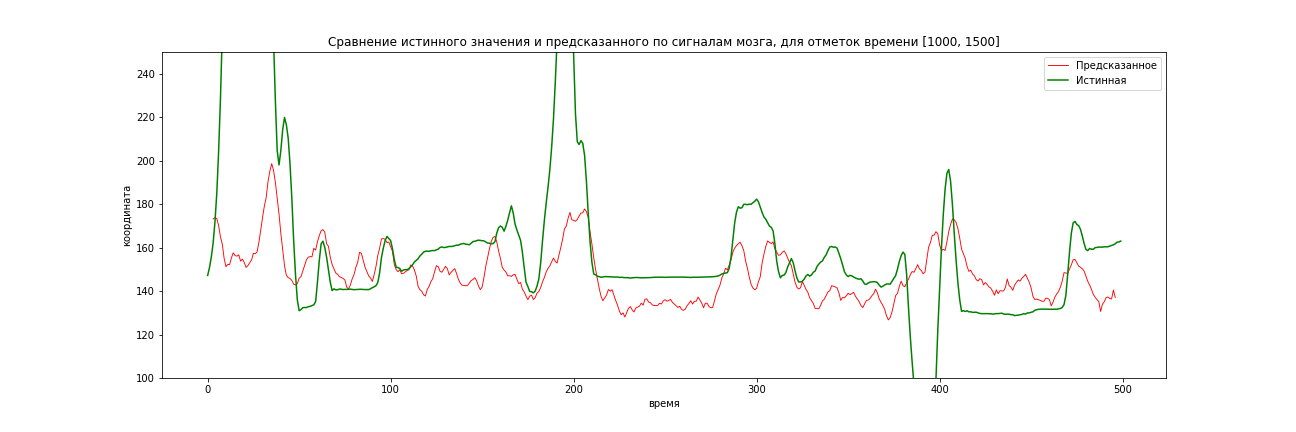
\includegraphics[scale=0.5]{images/1.png}
\end{figure}
\begin{figure}[H]
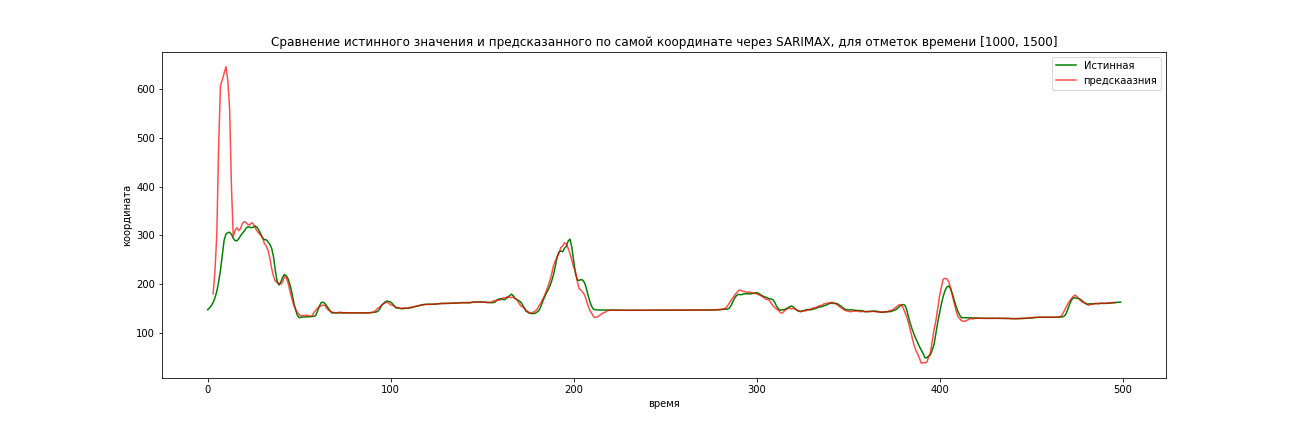
\includegraphics[scale=0.5]{images/2.png}
\end{figure}
\begin{figure}[H]
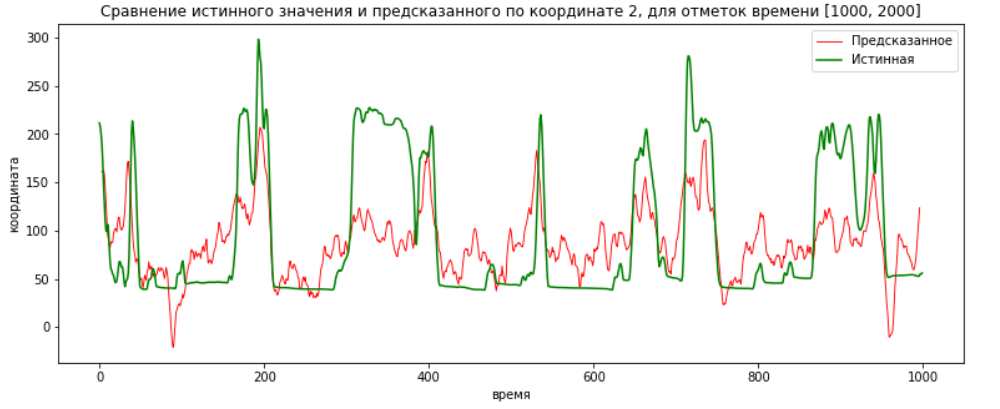
\includegraphics[scale=0.5]{images/3.png}
\end{figure}

Посмотрим на предсказания в 3D.
\begin{figure}[H]
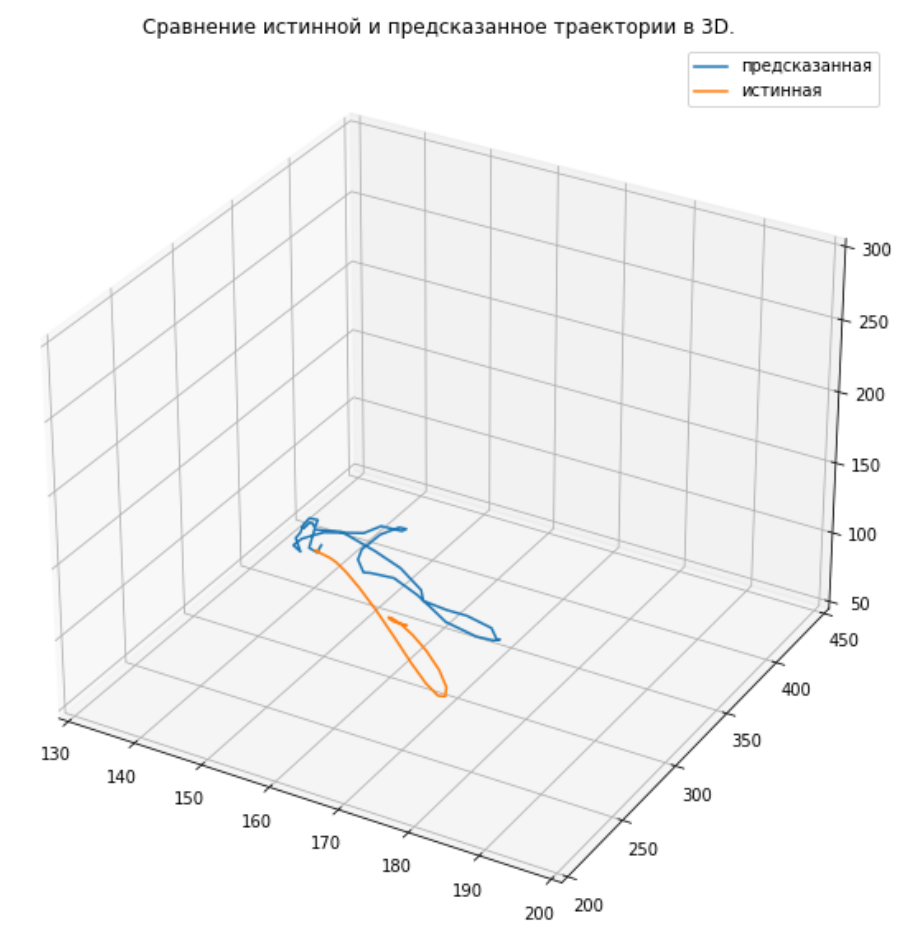
\includegraphics[scale=0.5]{images/4.png}
\end{figure}
И наконец, применим модель линейной регрессии.
\begin{figure}[H]
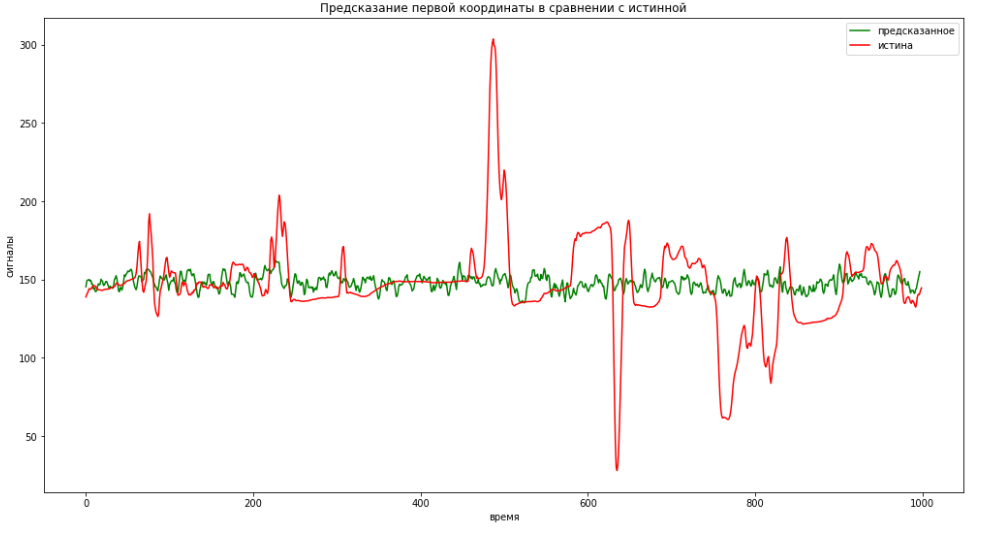
\includegraphics[scale=0.5]{images/5.png}
\end{figure}

Из графиков можно сделать вывод, что уже сейчас, используя только баловый алгоритм PLS удалось определять основные закономерности и пики в движении. Стоит отметить, что особенно хорошо определялись именно резкие изменения по координатам, а когда кисть не двигалась, предсказания были не точными и шумными. Это не удивительно, ведь когда мозг посылает сигналы руке, он думает не о кординате руки, а о силе, которую надо приложить мышце, то есть по второму закону Ньютона, об ускорении руки. Иными словами, при одинаковых сигналах мозга траектория движения руки будет одинаковая, не зависимо от того, находимся ли мы в точке $(0,0,0)$ или в точке $(100,100,100)$, так что предсказывать напрямую координату по сигналам мозга не совсем правильно. Кроме того, видно, что обычная линейная регрессия не добилась хоть каких-то результатов. Таким образом имеет смысл использовать алгоритмы понижения резмерности. В будущем предполагается оценить предсказания алгоритма по функциям риска, указанных выше.

\section{Сравнение моделей, анализ ошибок}
Рассматривается прогнозирование временного ряда координаты кисти, по прошлым точкам траектрии. Предлагается сравнить три модели --- $PLS$ в чистом виде, $SARIMAX$ в чистом виде и их микс. Сравнение происходит по метрикам $MSE, MAE$.
\begin{figure}[H]
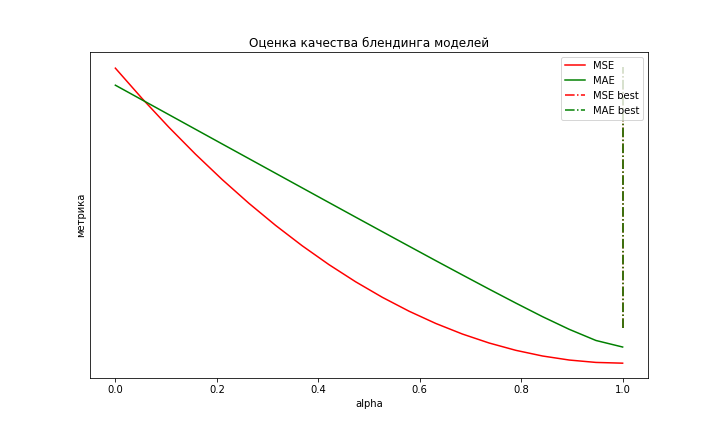
\includegraphics[scale=1]{images/6.png}
\end{figure}
Как видно, микс моделей показал наилучший результат.
\section{Заключение}



\nocite{*}
\bibliographystyle{plain}
\bibliography{references}



\end{document}
